\documentclass[PICOAPC.tex]{subfiles}

\begin{document}

\subsection{Gravitational Waves and Inflation}
\label{sec:inflation}

Measurements of the \ac{CMB} $BB$ angular power spectrum are the only foreseeable way to detect  inflationary gravitational waves. The strength of the signal, quantified by the tensor-to-scalar ratio $r$, is a direct measure of the expansion rate of the Universe during inflation, and together with the Friedmann equation, it reveals the energy scale of inflation. A detection of $r$  ``would be a watershed discovery'', a quote from the 2010 decadal panel report~\citep{blandford2010}. 
%\comred{do you need to explain what BB is?}

PICO will detect primordial gravitational waves if inflation occurred at an energy scale of at least $5\times 10^{15}\,\rm{GeV}$, or equivalently $r= 5\times 10^{-4} \, (5\sigma)$.  In a community white paper setting targets for measurements of inflationary gravitational waves in the next decade, \citet{Shandera_etal} quote two theoretically motivated targets: (1) rejecting $r=0.01$, and (2) rejecting $r=0.001$. The second threshold is motivated by the goal of rejecting all inflationary models that naturally explain the observed value of the spectral index of primordial fluctuations $n_{\rm s}$ and having a characteristic scale in the potential that is larger than the Planck scale. 
They write "If these thresholds are passed without a detection, most textbook models of inflation will be ruled out; and, while the possibility of an early inflationary phase would still remain viable, the data would then force a significant change in our understanding of the primordial Universe." PICO is the only next decade experiment with the raw sensitivity to reject both targets at high confidence; see Figure~\ref{fig:nsr}. It is the only next decade experiment that can detect inflationary models that have $r \geq 5\times 10^{-4}$ at high confidence. 

%A detection will provide evidence for a new energy scale tantalizingly close to the energy scale associated with grand unified theories, probe physics at energies far beyond the reach of terrestrial colliders, and be the first observation of a phenomenon associated with quantum gravity~\cite{Krauss:2013pha}. 

%There are only two classes of slow-roll inflation in agreement with current data that naturally explain the observed value of the spectral index of primordial fluctuations $n_{\rm s}$~\cite{Aghanim:2018eyx}. The first class is characterized by potentials of the form $V(\phi)\propto\phi^p$. The second class is characterized by potentials that approach a constant as a function of field value, either like a power law or exponentially. All models in this class, with a characteristic scale in the potential that is larger than the Planck scale, predict a tensor-to-scalar ratio of $r\gtrsim 0.001$.

%With its strong constraints on $r$, the strongest anticipated among any proposed next decade experiment, PICO will either detect gravitational waves from either of these classes with high confidence, or it will be the only experiment to answer the challenge articulated by the recent `Inflationary Gravitational Waves' community science paper: "If these thresholds are passed without a detection, most textbook models of inflation will be ruled out; and, while the possibility of an early inflationary phase would still remain viable, the data would then force a significant change in our understanding of the primordial Universe."~\cite{Shandera_etal}.


%The simplest models of inflation, in which there is a single inflaton field, predict primordial fluctuations that are very nearly Gaussian with $|f^{\rm local}_{\rm NL}| <1$, where $f^{\rm local}_{\rm NL}$ is a parameter quantifying the level of local non-Gaussianity~\citep{planck2015_17}. A detection of $|f^{\rm local}_{\rm NL}| >1$ points exclusively to models of inflation with multiple fields (Fig.~\ref{fig:fnlconstraint}). 
%For $f^{\rm local}_{\rm NL}=2$, $3\sigma$ evidence will be reached through correlations between the PICO lensing potential maps (\S~\ref{sec:gravitationallensing}) and LSST galaxies. If LSST's auto-correlation can only be used on smaller angular scales $L\ge 20$, the $3\sigma$ evidence weakens to $2\sigma$. 

%\begin{figure}[!thb]
%\centering
%\vspace{-0.05in}
%\hspace{-0.15in}
%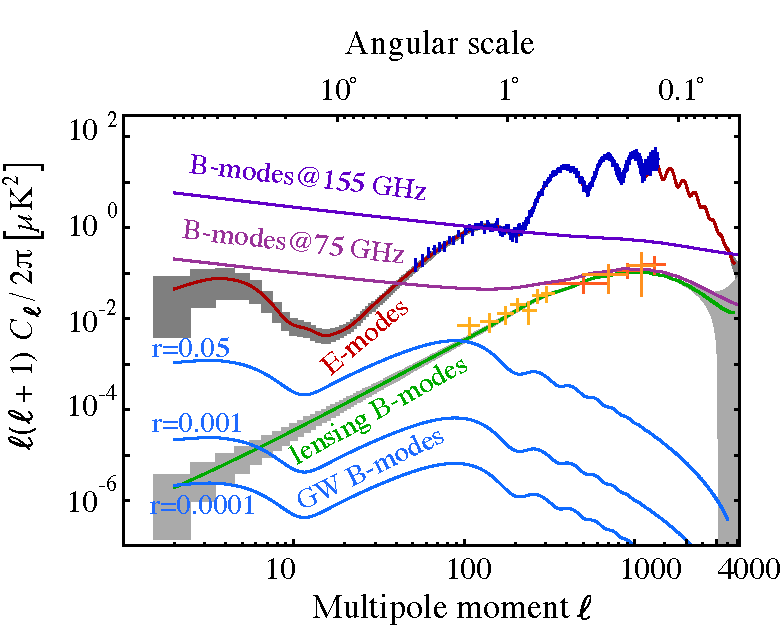
\includegraphics[width=3in]{images/cmb_powspec_PICOv4p1_v2.pdf}
%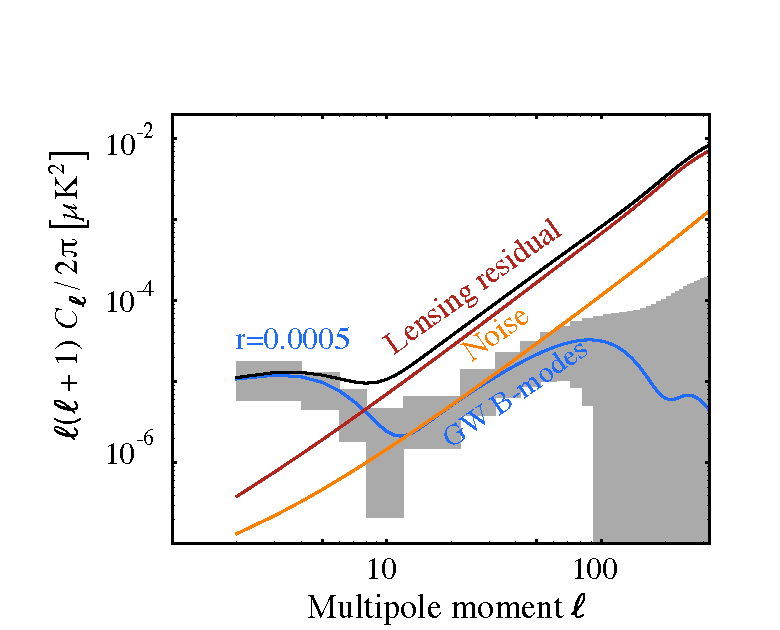
\includegraphics[width=3in]{images/cmbbb_powspec_PICOv4p1_v4.pdf}
%\vspace{-0.1in}
%\caption{\captiontext With PICO's baseline configuration we will measure the $EE$ (left, red) and lensing $BB$ (green) angular power spectra with high precision (grey). PICO's goal is to detect $r= 5\times 10^{-4}\, (5\sigma)$ (right, grey). This forecast includes PICO's 80\% delensing (red) and foreground separation. The baseline noise level (right, orange) allows detection of even lower levels; we expect foreground separation to limit performance.  As an example we show the total $BB$ spectra on the cleanest $60\%$ of the sky at 75 and 155~GHz (left, purple). The foregrounds largely dominate the cosmological signals. Also shown are measurements of lensing from current experiments (left, orange)~\citep{PB_BB, keisler2015, actpol_lensing_BB, Array:2015xqh}, \planck 's $EE$ measurements (left, dark blue)~\citep{Planck2018_I}, and the $BB$ spectrum produced by an inflationary gravity wave (GW) signal with different values of $r$ (cyan). 
%\label{fig:clbb} }
%\vspace{-0.05in}
%\end{figure}

\begin{figure}[!thb]
\parbox{4.5in}{\centerline{
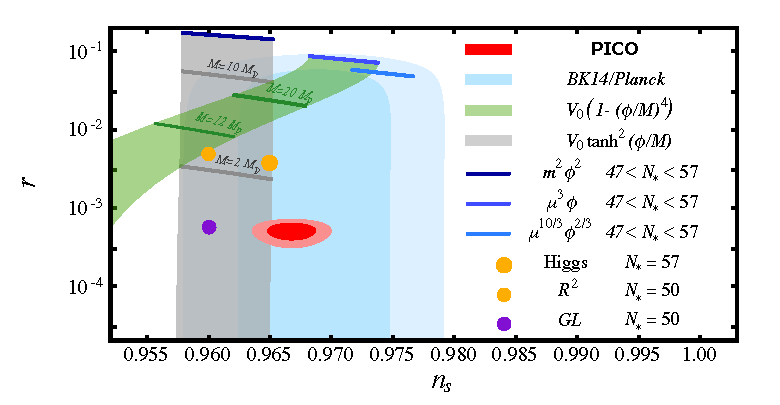
\includegraphics[width=4.5in]{images/nsrlabeledrp0005_PICOv2.pdf} } }
\parbox{1.8in}{
\caption{\captiontext  Current $1\sigma$ and 2$\sigma$ limits on $r$ and $n_{\rm s}$ (cyan) and forecasted constraints for a fiducial model with $r = 0.0005$ for PICO, together with predictions for selected models of inflation. Characteristic super-Planckian scales in the potentials are marked with darker lines. GL is the Goncharev-Linde model (see text). }
\label{fig:nsr}}
\vspace{-0.1in}
\end{figure}

%\paragraph{Observational Considerations}
%\noindent$\bullet$ {\bf Observational Considerations} \hspace{0.1in} 
%The $BB$ angular power spectrum measured by PICO will have contributions from Galactic sources of emission and `lensing' $B$-modes, created by gravitational lensing of $E$-modes as the CMB photons traverse the gravitational potentials throughout the Universe (Fig.~\ref{fig:clbb} and \S\,\ref{sec:gravitationallensing}).  In case of an $r$ detection, there will be two additional features due to the inflationary signal. One is the `recombination peak' at $\ell = 80$ and the other is the `reionization peak' at multipoles of $\ell\lesssim 10$. 

Uncertainty in the characterization of Galactic foregrounds already limits our ability to constrain $r$. These foregrounds 
are anticipated to be nearly 1000 times stronger than next-decade-targeted inflationary $B$-mode signals at low $\ell$ multipoles. %$\ell=8$. 
`Lensing' $B$-modes, created by gravitational lensing of $E$-modes, are an additional effective foreground for the higher multipoles. With sufficiently high resolution to remove at least 73\% of the lensing effects, and 21 frequency bands to account for foregrounds, no other next-decade experiment is better equipped than PICO to overcome the challenges in robustly finding the faint inflationary signal, or in rejection confusion due to foregrounds. 

%as the CMB photons traverse the gravitational potentials throughout the Universe, are en effective foreground for the inflationary $BB$ signal at $\ell=80$.  
% (Fig.~\ref{fig:clbb} and \S\,\ref{sec:gravitationallensing}).
%PlCO has the angular resolution to remove 73\% of the lensing $B$-mode power, assuming strong foregrounds, and the frequency coverage to remove foregrounds to levels below the $B$-mode reionization peak; see Section~\ref{sec:??}. 
%If an inflationary $B$-mode signal is detected, it is important to characterize its entire $\ell$ dependence in the predicted reionization and  recombination peaks, in order to confirm -- rather than assume -- its expected dependence on angular scale.  Furthermore, the PICO full-sky coverage will enable detection of the recombination peak in several independent patches of the sky, giving an important systematic cross-check. Only PICO can provide these important benefits. 

\subsection{Fundamental Particles and Fields} %: Light Relics, Dark Matter, and Neutrinos}
\label{sec:relics_neutrinos}

%%%%%%%%%%%%%%%%%%%%%%%%%
$\bullet$ {\bf Light Relics} \hspace{0.1in} The `effective number of light relic particle species' $\Neff$ gives information about particle species that are predicted to have existed in the early Universe in extensions of the Standard Model. The canonical value with three neutrino families is $\Neff = 3.046$. Additional light particles contribute a change $\Delta \Neff$ that is a function only of the decoupling temperature of the additional species and the spin of the particle~$g$. PICO will provide a constraint $\Delta \Neff < 0.06 \, (95\%)$ and will either detect new particle species, or constrain the lowest temperature $T_{F}$ at which any vector particle (spin 1) could have fallen out of equilibrium to a factor of 400 higher than today's constraint. No other next decade experiment will provide a tighter constraint. \comred{add Neff white paper, and check the statement.}  \\ %(Fig.~\ref{fig:Neff_future}, right). 
\noindent$\bullet$ {\bf Neutrino Mass} \hspace{0.1in} \label{neutrino_fundamental} The origin, structure, and values of the neutrino masses are among the great outstanding  questions about the nature of the Standard Model particles.  
%Cosmology offers a  measurement of the sum of the neutrino masses $\sum m_\nu$ through the gravitational influence of the non-relativistic  cosmic neutrinos, specifically the suppression of cosmic structure power on small spatial scales, which PICO will measure via CMB lensing (\S~\ref{sec:gravitationallensing}). 
All cosmological measurements of $\sum m_\nu$ relate the amplitudes of the matter power spectrum and the primordial fluctuation power spectrum $A_s$.  Both are limited by degeneracies; the former is limited by our knowledge of $\omega_m$ and the latter by the optical depth to reionization $\tau$. PICO is the only instrument that will self consistently provide three of these four ingredients: $\tau$, $A_s$ from the primary CMB, and the matter power spectrum via CMB lensing. In combination with $\omega_m$ coming from DESI and EUCLID data, PICO will give $\sigma(\sum m_\nu) = 14$ meV, giving a $4\,\sigma$ detection of the minimum sum of 58~meV.
PICO will measure  $\sum m_\nu$ in two additional ways, which will give equivalent constraints. 

%The current measurement of $\Neff = 2.99 \pm 0.17$~\citep{Planck2018_VI} already confirms the existence of these neutrinos at $>10\sigma$ and their mass implies that they will contribute to the matter density at low redshifts.  The best current mass constraint arises from a combination of  \planck~and BOSS \ac{BAO} giving $\sum m_\nu < 0.12$ eV (95\%) \cite{Planck2018_VI}.

%Cosmological measurements are primarily sensitive to the suppression of power on small scales after the neutrinos become non-relativistic, which can be measured via CMB lensing (\S~\ref{sec:gravitationallensing}), or weak lensing in galaxy surveys.  However, these measurements are limited by our knowledge of the amplitude of the primordial fluctuation power spectrum $A_s$ because they only constrain the combination $A_s e^{-2 \tau}$, where $\tau$ is the optical depth to reionization. Although many astrophysical surveys hope to detect $\sum m_\nu$, any detection of the minimum value expected from particle physics, $\sum m_\nu = 58$~meV, at more than $2 \sigma$, will require a better measurement of $\tau$.
% and thus do not provide a high-precision measurement of either $A_s$ or $\tau$ separately.  \comor{we mention 'galaxy survey', but don't complete the thread of thought. Do we mean to say that the galaxy survey will be limited by the same degeneracy?}

%The strongest constraints on $\tau$ come from the $EE$ spectrum at $\ell < 10$, which requires measurements over the largest angular scales  and good separation of Galactic foreground sources of emission. The best current measurement with $\sigma({\tau}) = 0.007$ is from \planck~\cite{Planck2018_VI}. With this uncertainty in $\tau$ one is limited to  $\sigma(\sum m_\nu) \gtrsim 25$ meV, after including forthcoming \ac{BAO} information (Fig.~\ref{fig:DM_baryons}, right); no other survey or cosmological probe will improve this constraint, unless a more accurate measurement of $\tau$ is made. One of the S3 experiments is attempting to measure the lowest $\ell$s and improve upon the \planck\ precision by a factor of about two~\citep{class}. A space mission with its access to the entire sky and broad frequency coverage is the most suitable platform for the measurement~(\S~\ref{sec:signal_separation} and \S~\ref{sec:complementarity}). PICO will reach the cosmic-variance limit uncertainty on $\tau$, $\sigma(\tau) = 0.002$~(\S~\ref{sec:luminoussources}), and using its deep CMB lensing map (\S~\ref{sec:gravitationallensing}) will therefore reach $\sigma(\sum m_\nu) = 14$ meV when combined with measurements of \ac{BAO} from DESI or Euclid~\cite{Levi:2013gra}.
%(without \ac{BAO} data the constraint is $\sigma(\sum m_\nu) = 43$ meV).
%This measurement will give a $4\sigma$ detection of the minimum sum (SO3). 

%Robustly detecting neutrino mass at  $> 3\sigma$ in any cosmological setting is only possible with an improved measurement of $\tau$, like the one achievable with PICO. This measurement will give $\sum m_\nu>0$ at greater than $4\sigma$ or would exclude the inverted hierarchy ($\sum m_\nu > 100$ meV) at 95\% confidence, depending on the central value of the measurement.  Lab-based measurement could determine the hierarchy before PICO, but only cosmology can measure $\sum m_\nu$.


%While our theoretical target for $\Neff$ is defined by particles that decoupled long before neutrinos did, there are a number of well-motivated scenarios in which the thermal evolution of the Standard Model is altered after the time of neutrino decoupling.  These scenarios will change the relationship between $\Neff$ as measured in the CMB and the value of $\Neff$ that affects the primordial abundance of the helium fraction $Y_p$ as inferred from big bang nucleosynthesis calculations. 
%While our theoretical target for $\Neff$ is defined by particles that decoupled long before neutrinos did, there are a number of well-motivated scenarios in which the thermal evolution of the Standard Model is altered after the time of neutrino decoupling.  These scenarios will change the relationship between $\Neff$ as measured in the CMB relative to the value of $\Neff$ that affects big bang nucleosynthesis calculations and the production of helium, which is quantified through the helium fraction $Y_p$.  
%For example, the decay of a thermal relic into photons after nucleosynthesis would reduce $\Neff$ in the CMB but could leave $Y_p$ unaltered from its Standard Model value.  PICO will make a simultaneous measurement of $\Neff$ and $Y_p$ with $\sigma(\Neff) = 0.08$ and $\sigma(Y_p) =0.005$, giving a 2\% uncertainty on the value of $Y_p$. These uncertainties are equivalent to those available with other astrophysical measurements, but the systematic uncertainties are entirely different. Systematic uncertainties currently limit our knowledge of $Y_{p}$. 

%%%%%




\noindent$\bullet$ {\bf Dark Matter} \hspace{0.1in} Cosmological measurements have already confirmed the existence of one relic that lies beyond the Standard Model: dark matter. \ac{CMB} experiments are effective in constraining dark matter candidates in the lower mass range, which is not available for terrestrial direct detection experiments~\citep{Slatyer2009,Galli2009,Huetsi2009,Huetsi2011,Madhavacheril:2013cna,Green:2018pmd}. 

PICO's constraining power comes from making high \ac{SNR} maps of the lensing-induced deflections of polarized photons, and cosmic-variance limited determinations of the $TT$, $TE$ and $EE$ spectra up to $\ell \simeq 2500$. 
For a spin-independent velocity-independent contact-interaction between dark matter and protons, chosen as our fiducial model, PICO will improve upon \planck 's dark matter cross-section constraints by a factor of 25 over a broad range of candidate dark matter masses that are largely unavailable for traditional direct detection experiments. %(Fig.~\ref{fig:DM_baryons}, right). 
If 2\% of the total dark content is made of axions, PICO's measurement of the $TT$, $TE$ and $EE$ spectra with additional constraints from the lensing reconstruction will detect this species at between $7$ and $13\sigma$, depending on the mass range. %, as shown in Figure~\ref{fig:axions}. 
This is an average improvement of a factor of 10 relative to \planck .


 
%PICO's constraining power comes primarily from making high \ac{SNR} maps of the lensing-induced deflections of polarized photons, which are discussed in Section~\ref{sec:extragalacticsci}.  For a spin-independent velocity-independent contact-interaction, chosen as our fiducial model, PICO will improve upon \planck 's dark matter cross-section constraints by a factor of 25 over a broad range of candidate masses that are largely unavailable for traditional direct detection experiments.


% (Fig.~\ref{fig:DM_baryons}, right). 
%The constraints are complementary to those forthcoming from direct detection experiments, which are more sensitive at the high mass range.  
%\comor{need to decide what to do with this section.}
%which is largely unavailable to traditional direct detection experiments

%\begin{figure}[t]
%\begin{center}
%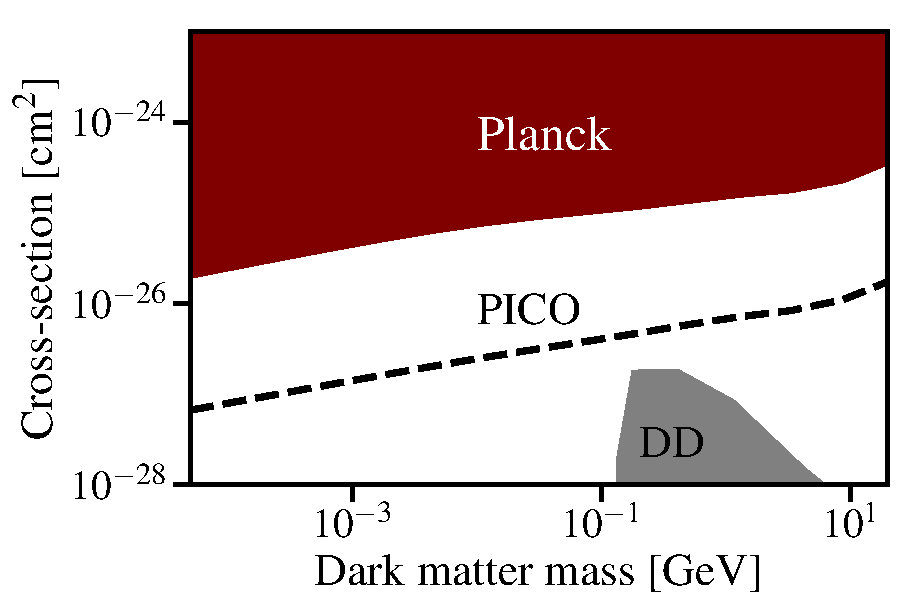
\includegraphics[width=0.50\textwidth]{images/pico_dd4.pdf}
%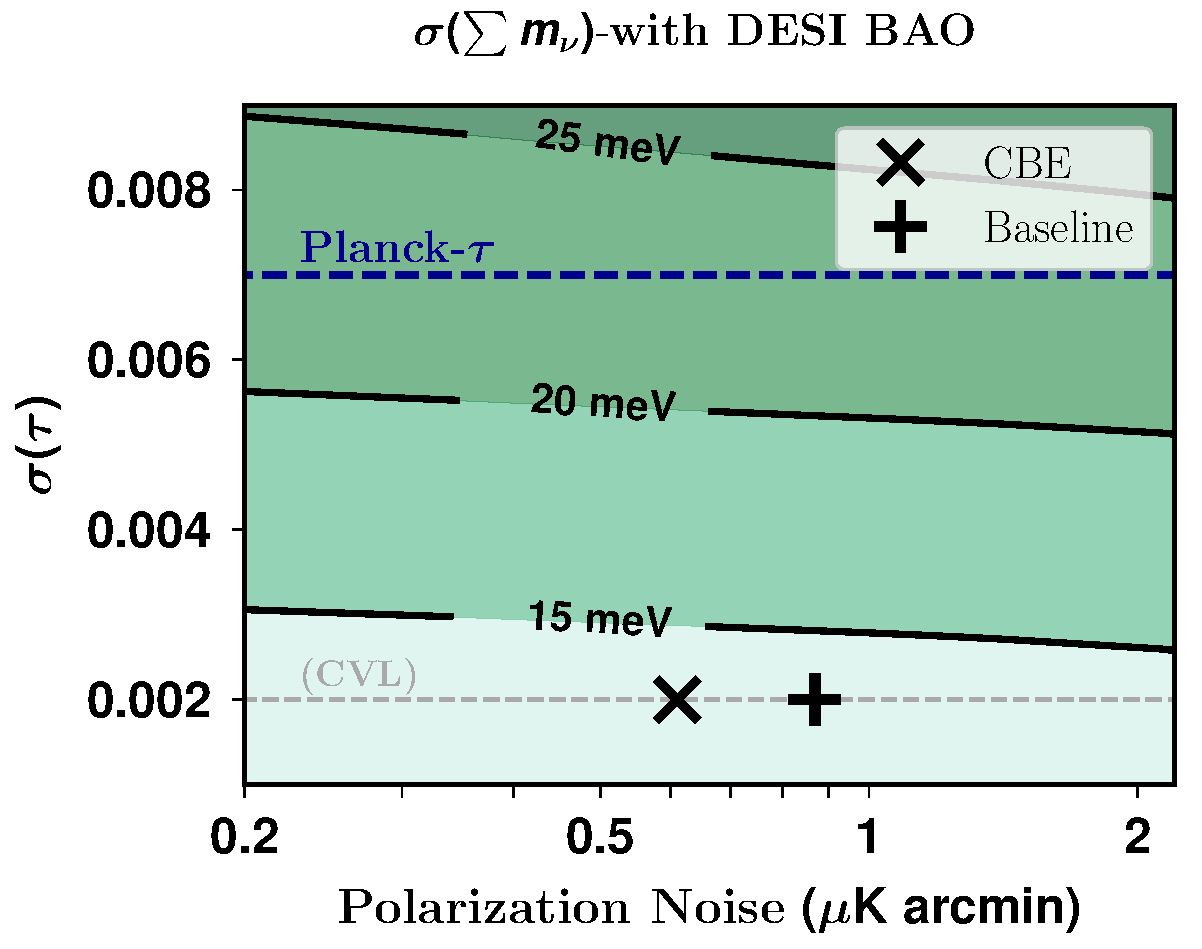
\includegraphics[width=0.48\textwidth]{images/Mnu_tauprior_final.pdf}
%\vspace{-0.15in}
%\caption{\captiontext {\bf Left:} PICO will give a factor of 25 more stringent constraint on the spin-independent velocity-independent dark matter scattering cross-section (dashed) relative to current \planck\ 95\% confidence limit (red)~\citep{2018PhRvL.121h1301G}. Terrestrial direct detection experiments are expected to give complementary and stronger constraints, but only for the higher dark matter masses (grey)~\cite{2018PhRvD..97l3013K}. 
%{\bf Right:} Using a cosmic-variance-limited (CVL) measurement of $\tau,\, \sigma(\tau)=0.002$, \ac{BAO} information from DESI, and separation of foregrounds over 70\% of the sky, PICO will reach $\sigma(\Sigma m_{\nu}) = 14$~meV (contours), giving at least a $4\sigma$ detection of the minimal expected sum of neutrino masses $\Sigma m_{\nu} = 58$~meV. 
%\label{fig:DM_baryons} }
%\end{center}
%\vspace{-0.2in}
%\end{figure}
%

%The axion is another dark matter candidate that is well motivated by string theory~\citep{Arvanitaki_etal} and that is consistent with straightforward extensions of the Standard Model of particle physics~\citep{peccei,weinberg,wilczek}. For an axion mass in the intermediate range $10^{-30} < m_a< 10^{-26} $~eV, current measurements constrain its fraction to be $\le 2$\% $(1\sigma)$ of the total dark-matter density. If 2\% of the total dark content is made of axions, PICO's measurement of the $TT$, $TE$ and $EE$ spectra with additional constraints from the lensing reconstruction will detect this species at between $7$ and $13\sigma$, depending on the mass range. %, as shown in Figure~\ref{fig:axions}. 
%This is an average improvement of a factor of 10 relative to \planck .
% and a factor of two relative to the combination of \planck\ and S3, respectively, profoundly shaping our understanding of the nature of dark matter and its small-scale clustering. 


%%%%%%%%%%%%%%%%%%%%%%%%%

%\subsection{Fundamental Fields: Primordial Magnetic Fields and Cosmic Birefringence}

$\bullet$ {\bf Primordial Magnetic Fields} \hspace{0.1in} One of the long-standing puzzles in astrophysics is the origin of observed 1--10~$\mu$G galactic magnetic fields~\citep{Widrow:2002ud}. Producing such fields through a dynamo mechanism requires a primordial seed field~\citep{Widrow:2011hs}. Moreover, $\mu$G-strength fields have been observed in proto-galaxies that are too young to have gone through the number of revolutions necessary for the dynamo to work~\citep{Athreya:1998}. A primordial magnetic field (PMF), present at the time of galaxy formation, could provide the seed or even eliminate the need for the dynamo altogether. Specifically, a 0.1~nG field in the intergalactic plasma would be adiabatically compressed in the collapse to form a $\sim$1~$\mu$G galactic field~\citep{Grasso:2000wj}.
PMFs could have been generated in the aftermath of phase transitions in the early Universe~\citep{Vachaspati:1991nm}, during inflation~\cite{Turner:1987bw,Ratra:1991bn}, or at the end of inflation~\cite{DiazGil:2007dy}. A detection of PMFs with the CMB would be a major discovery because it would establish the magnetic field's primordial origin, signal new physics beyond standard models of particle physics and cosmology, and discriminate among different theories of the early Universe~\cite{Barnaby:2012tk,Long:2013tha,Durrer:2013pga}.

%The current CMB bounds on PMF strength are $B_{\rm 1\,Mpc}<1.2$ nG at 95\% CL for the scale-invariant~PMF spectrum \cite{Planck2015PMF,Kunze2015,Chluba2015PMF,Zucca:2016iur}, based on measurements of the $TT$, $TE$, $EE$, and $BB$ spectra.\footnote{It is conventional to quote limits on the PMF strength smoothed over a $1$~Mpc region in comoving units,  i.e., rescaled to $z=0$: $\mathbf{B}_{\rm today} = a^2\mathbf{B}(a)$.} 
%In particular, PMF sourced vector modes contribute to the $BB$ power spectrum at high $\ell$ \cite{Lewis:2004ef}. 
%The much more accurate measurement of $BB$ by PICO would only marginally improve the PMF bound because CMB spectra scale as $B^4_{\rm 1\,Mpc}$. However, Faraday rotation provides a signature that scales linearly with the strength of PMFs~\cite{Kosowsky:1996yc}. It converts CMB $E$ modes into $B$ modes, generating mode-coupling $EB$ and $TB$ correlations. So far this signature has been out of reach because prior experiments did not have sufficient sensitivity. 

Using Faraday rotation measurements, PICO will probe PMFs as weak as 0.1~nG ($1\sigma$), a precision that already includes the effects of imperfect lensing subtraction, Galactic foregrounds~\cite{Oppermann:2011td,De:2013dra,Pogosian:2013dya}, and other systematic effects. With this precision, which is a factor of five stronger than achievable with \comred{S3} experiments, PICO can conclusively rule out the purely primordial (i.e., no-dynamo driven) origin of the largest galactic magnetic fields. \\
%
$\bullet$ {\bf Cosmic Birefringence} \hspace{0.1in}
A number of well-motivated extensions of the Standard Model involve fields with parity-violating coupling~\citep{Freese:1990rb,Frieman:1995pm,Carroll:1998zi,Kaloper:2005aj,Carroll:1998zi,2008PhRvL.101n1101C,Gluscevic:2010vv}. Their presence may cause cosmic birefringence -- a rotation of the polarization of an electromagnetic wave as it propagates across cosmological distances~\cite{Harari:1992ea,Carroll:1989vb,Carroll:1998zi}.
Cosmic birefringence converts primordial $E$-modes into $B$-modes, producing $TB$ and $EB$ cross-correlations whose magnitude depends on the statistical properties of the rotation field in the sky~\cite{Kamionkowski:2008fp,Gluscevic:2009mm,Gluscevic:2012me}.
Using the combination of five bands in the 70--156~GHz range, PICO will reduce the 95\% CL bound on uniform rotation angle by a factor of 300 to 0.1\arcmin ;   The 95\% CL bound on the amplitude of a scale-invariant rotation spectrum will be reduced by a factor of 275 to $4\times10^{-4}$~deg$^2$. These will give constraints on extensions of the Standard Model and on string-theory-motivated axions~\cite{Svrcek:2006yi,Pospelov:2008gg}.




%(nearly) massless axion-like pseudo-scalar fields coupled to photons via the Chern-Simons interaction term~\citep{Freese:1990rb,Frieman:1995pm,Carroll:1998zi,Kaloper:2005aj}. These couplings also generically arise within quintessence models for dark energy~\citep{Carroll:1998zi}, chiral-gravity models~\citep{2008PhRvL.101n1101C}, and models that produce parity-violation during inflation~\cite{Gluscevic:2010vv}. Regardless of the source of the parity-violating coupling, its presence may cause cosmic birefringence -- a rotation of the polarization of an electromagnetic wave as it propagates across cosmological distances~\cite{Harari:1992ea,Carroll:1989vb,Carroll:1998zi}. Cosmic birefringence converts primordial $E$-modes into $B$-modes, producing $TB$ and $EB$ cross-correlations whose magnitude depends on the statistical properties of the rotation field in the sky~\cite{Kamionkowski:2008fp,Gluscevic:2009mm,Gluscevic:2012me}. Previous studies have constrained both a uniform rotation angle as well as anisotropic rotation described by a power spectrum \cite{Gluscevic:2012me}. The current bound on a uniform angle is 30\arcmin\ (68\%)~\cite{Planck2016_XLIX}, and the bound on the amplitude of a scale-invariant rotation angle spectrum, which could be caused by fluctuations in a light pseudo-scalar field present during inflation~\cite{Pospelov:2008gg}, is 0.11~deg$^2$ (95\%)~\citep{Array:2017rlf}). Using the combination of five bands in the 70--156~GHz range, PICO will reduce the 95\% CL bound on the uniform rotation angle by a factor of 300, to 0.1\arcmin.  
%, assuming that the beam can be calibrated to reach the main science goals without \emph{assuming} vanishing parity-odd spectra of $EB$ and $TB$ type. 
%The 95\% CL bound on the amplitude of a scale-invariant rotation spectrum will be reduced by a factor of 275 to $4\times10^{-4}$~deg$^2$, giving important constraints on string-theory-motivated axions~\cite{Svrcek:2006yi,Pospelov:2008gg}.

%A number of well-motivated extensions of the Standard Model involve (nearly) massless axion-like pseudo-scalar fields coupled to photons via the Chern-Simons interaction term~\citep{Freese:1990rb,Frieman:1995pm,Carroll:1998zi,Kaloper:2005aj}. These couplings also generically arise within quintessence models for dark energy~\citep{Carroll:1998zi}, chiral-gravity models~\citep{2008PhRvL.101n1101C}, and models that produce parity-violation during inflation~\cite{Gluscevic:2010vv}. Regardless of the source of the parity-violating coupling, its presence may cause cosmic birefringence -- a rotation of the polarization of an electromagnetic wave as it propagates across cosmological distances~\cite{Harari:1992ea,Carroll:1989vb,Carroll:1998zi}. Cosmic birefringence converts primordial $E$-modes into $B$-modes, producing $TB$ and $EB$ cross-correlations whose magnitude depends on the statistical properties of the rotation field in the sky~\cite{Kamionkowski:2008fp,Gluscevic:2009mm,Gluscevic:2012me}. Previous studies have constrained both a uniform rotation angle as well as anisotropic rotation described by a power spectrum \cite{Gluscevic:2012me}. The current bound on a uniform angle is 30\arcmin\ (68\%)~\cite{Planck2016_XLIX}, and the bound on the amplitude of a scale-invariant rotation angle spectrum, which could be caused by fluctuations in a light pseudo-scalar field present during inflation~\cite{Pospelov:2008gg}, is 0.11~deg$^2$ (95\%)~\citep{Array:2017rlf}). Using the combination of five bands in the 70--156~GHz range, PICO will reduce the 95\% CL bound on the uniform rotation angle by a factor of 300, to 0.1\arcmin.  
%, assuming that the beam can be calibrated to reach the main science goals without \emph{assuming} vanishing parity-odd spectra of $EB$ and $TB$ type. 
%The 95\% CL bound on the amplitude of a scale-invariant rotation spectrum will be reduced by a factor of 275 to $4\times10^{-4}$~deg$^2$, giving important constraints on string-theory-motivated axions~\cite{Svrcek:2006yi,Pospelov:2008gg}.


\end{document}

